\documentclass{standalone}
\usepackage{tikz}
\usepackage{hsbcommon}
\begin{document}
    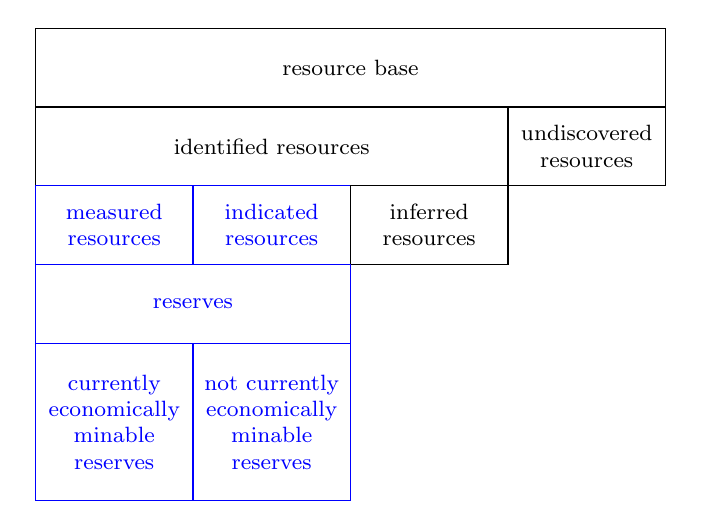
\begin{tikzpicture}\footnotesize
    \begin{scope}[black]
        \draw (0,0)   rectangle node  {resource base}  (8,-1);
        \draw (0,-1)   rectangle node  {identified resources}  (6,-2);
        \draw (6,-1)   rectangle node  {
            \parbox{2cm}{\centering undiscovered resources}
        }  (8,-2);
        \draw[blue] (0,-2)   rectangle node  {
            \parbox{2cm}{\centering measured resources}
        }  (2,-3);
        \draw[blue] (2,-2)   rectangle node  {
            \parbox{2cm}{\centering indicated resources}
        }  (4,-3);
        \draw (4,-2)   rectangle node  {
            \parbox{2cm}{\centering inferred resources}
        }  (6,-3);
    \end{scope}
    \begin{scope}[blue]
        \draw (0,-3)   rectangle node  {
            \parbox{2cm}{\centering reserves}
        }  (4,-4);
        \draw (0,-4)   rectangle node  {
            \parbox{2cm}{\centering currently economically minable reserves}
        }  (2,-6);
        \draw (2,-4)   rectangle node  {
            \parbox{2cm}{\centering not currently economically minable reserves}
        }  (4,-6);
    \end{scope}
    \end{tikzpicture}
\end{document}